\documentclass[12pt]{report}

% --- Idioma y codificación ---
\usepackage[spanish]{babel}
\usepackage[utf8]{inputenc}

% --- Matemáticas ---
\usepackage{amsmath, amssymb, amsthm}

% --- Gráficos y figuras ---
\usepackage{graphics, graphicx, subfigure}
\usepackage{tikz, pgffor, ifthen}

% --- Tablas y estructuras ---
\usepackage{array, multicol, longtable, booktabs}

% --- Listas y enumeraciones ---
\usepackage{enumerate, enumitem}

% --- Márgenes y geometría ---
\usepackage[a4paper, margin=1.5cm]{geometry}

% --- Diseño y marco ---
\usepackage[framemethod=TikZ]{mdframed}

% --- Texto y contenido de prueba ---
\usepackage{lipsum}

\usepackage{subfiles}

% --- Hipervínculos ---
\usepackage{hyperref}
\hypersetup{
    colorlinks=true,
    linkcolor=black,
    filecolor=magenta,
    urlcolor=cyan
}

% --- Código fuente (listings) ---
\usepackage{listings}
\usepackage{xcolor}

\definecolor{listing-background}{HTML}{F7F7F7}
\definecolor{listing-rule}{HTML}{B3B2B3}
\definecolor{listing-numbers}{HTML}{B3B2B3}
\definecolor{listing-text-color}{HTML}{000000}
\definecolor{listing-keyword}{HTML}{435489}
\definecolor{listing-keyword-2}{HTML}{1284CA}
\definecolor{listing-keyword-3}{HTML}{9137CB}
\definecolor{listing-identifier}{HTML}{435489}
\definecolor{listing-string}{HTML}{00999A}
\definecolor{listing-comment}{HTML}{8E8E8E}

\lstdefinestyle{myStyle}{
    language=C++,
    alsolanguage=scala,
    numbers=left,
    xleftmargin=2.7em,
    framexleftmargin=2.5em,
    backgroundcolor=\color{gray!15},
    basicstyle=\color{listing-text-color}\linespread{1.0}\ttfamily,
    breaklines=true,
    frameshape={RYR}{Y}{Y}{RYR},
    rulecolor=\color{black},
    tabsize=2,
    numberstyle=\color{listing-numbers}\linespread{1.0}\small\ttfamily,
    aboveskip=1.0em,
    belowskip=0.1em,
    abovecaptionskip=0em,
    belowcaptionskip=1.0em,
    keywordstyle={\color{listing-keyword}\bfseries},
    keywordstyle={[2]\color{listing-keyword-2}\bfseries},
    keywordstyle={[3]\color{listing-keyword-3}\bfseries\itshape},
    sensitive=true,
    identifierstyle=\color{listing-identifier},
    commentstyle=\color{listing-comment},
    stringstyle=\color{listing-string},
    showstringspaces=false,
    label=lst:bar,
    captionpos=b
}
\lstset{style=myStyle}

% --- Marca de agua ---
\usepackage{eso-pic}
\AddToHook{shipout/foreground}{
    \begin{tikzpicture}[remember picture,overlay]
        \node at (current page.center){
            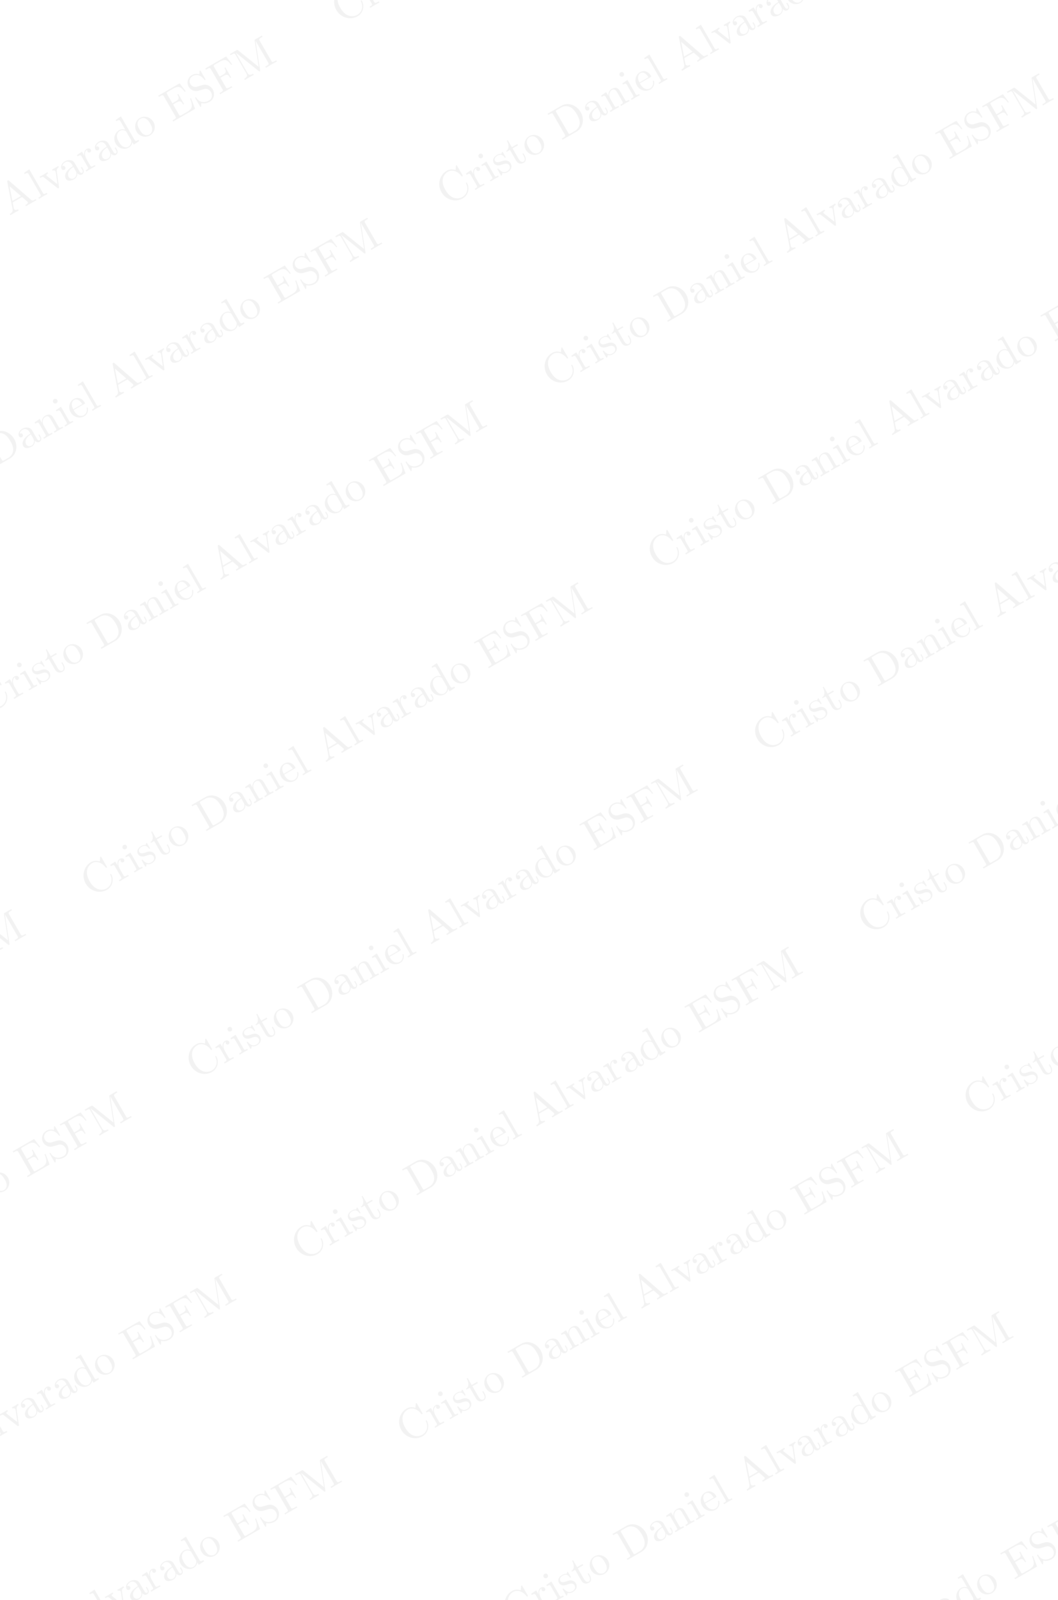
\includegraphics[width=\paperwidth,height=\paperheight,keepaspectratio]{watermark-1.png}
        };
    \end{tikzpicture}
}

% --- Redefiniciones de encabezados de capítulo y sección ---
\makeatletter
% Capítulo (estilo original conservado)
\def\@makechapterhead#1{%
  {\parindent \z@ \raggedright
    \reset@font
    \hrule
    \vspace*{10\p@}%
    \par
    \center \LARGE \scshape \@chapapp{} \huge \thechapter
    \vspace*{10\p@}%
    \par\nobreak
    \vspace*{10\p@}%
    \par
    \vspace*{1\p@}%
    \hrule
    \vspace*{30\p@}  % Espaciado reducido
    \centering\Huge \scshape #1\par\nobreak  % Centrado y scshape
    \vskip 30\p@  % Espaciado reducido
  }}


% Sección
\renewcommand{\section}{\@startsection{section}{1}{\z@}%
  {-2.5ex \@plus -0.5ex \@minus -0.1ex}%  % Espaciado superior reducido
  {1ex \@plus 0.1ex}%                     % Espaciado inferior reducido
  {\normalfont\Large\sectionstyle}}
\newcommand{\sectionstyle}[1]{%
  \par\noindent\hrule
  \vspace{0.2ex}%   % Espaciado entre líneas reducido
  {\scshape{#1}\par}%  % Centrado perfecto y scshape
  \vspace{0.4ex}%   % Espaciado entre líneas reducido
  \hrule
}

% Subsección
\renewcommand{\subsection}{\@startsection{subsection}{2}{\z@}%
  {-2ex \@plus -0.4ex \@minus -0.1ex}%  % Espaciado superior reducido
  {0.8ex \@plus 0.1ex}%                 % Espaciado inferior reducido
  {\normalfont\large\subsectionstyle}}
\newcommand{\subsectionstyle}[1]{%
  \par\noindent\hrule
  \vspace{-0.4ex}%  % Espaciado entre líneas reducido
  {\scshape #1\par}%  % Centrado perfecto y scshape
  \vspace{0.4ex}%  % Espaciado entre líneas reducido
  \hrule
}

% Subsubsección
\renewcommand{\subsubsection}{\@startsection{subsubsection}{3}{\z@}%
  {-1.5ex \@plus -0.3ex \@minus -0.1ex}%  % Espaciado superior reducido
  {0.5ex \@plus 0.1ex}%                   % Espaciado inferior reducido
  {\normalfont\normalsize\subsubsectionstyle}}
\newcommand{\subsubsectionstyle}[1]{%
  \par\noindent\hrule
  \vspace{0.4ex}%   % Espaciado entre líneas reducido
  {\scshape #1\par}%  % Centrado perfecto y scshape
  \vspace{0.4ex}%   % Espaciado entre líneas reducido
  \hrule
}
\makeatother

% --- Entornos personalizados ---
% (aquí puedes definir tus theorems, definiciones, etc.)


% --- Entornos personalizados ---
\newtheoremstyle{largebreak}{}{ }{\normalfont}{}{\bfseries}{}{\newline}{}
\theoremstyle{largebreak}

\newmdtheoremenv[hidealllines=true,roundcorner=5pt,backgroundcolor=gray!60!red!30]{exa}{Ejemplo}[section]
\newmdtheoremenv[hidealllines=true,roundcorner=5pt,backgroundcolor=gray!50!blue!30]{obs}{Observaci\'on}[section]
\newmdtheoremenv[hidealllines=true,roundcorner=5pt,backgroundcolor=green!50!blue!30]{preg}{Pregunta}[section]
\newmdtheoremenv[hidealllines=true,roundcorner=5pt,backgroundcolor=yellow!40]{idea}{Idea}[section]
\newmdtheoremenv[rightline=false,leftline=false]{theor}{Teorema}[section]
\newmdtheoremenv[rightline=false,leftline=false]{propo}{Proposici\'on}[section]
\newmdtheoremenv[rightline=false,leftline=false]{cor}{Corolario}[section]
\newmdtheoremenv[rightline=false,leftline=false]{lema}{Lema}[section]
\newmdtheoremenv[roundcorner=5pt,backgroundcolor=gray!30,hidealllines=true]{mydef}{Definici\'on}[section]
\newmdtheoremenv[roundcorner=5pt]{excer}{Ejercicio}[section]

% --- Comandos auxiliares ---
\def\proof{\paragraph{Demostraci\'on:\\}}
\def\endproof{\hfill$\blacksquare$}
\def\sol{\paragraph{Soluci\'on:\\}}
\def\endsol{\hfill$\square$}

\newcommand\abs[1]{\ensuremath{\left|#1\right|}}
\newcommand\divides{\ensuremath{\bigm|}}
\newcommand\cf[3]{\ensuremath{#1:#2\rightarrow#3}}
\newcommand\contradiction{\ensuremath{\#_c}}
\newcommand\natint[1]{\ensuremath{\left[\big|#1\big|\right]}}

\newcounter{figcount}
\setcounter{figcount}{1}

\renewcommand{\lstlistingname}{Código}
\renewcommand{\lstlistlistingname}{Lista de \lstlistingname s}

% --- Comienzo del documento ---
\begin{document}
    \setlength{\parskip}{5pt}
    \setlength{\parindent}{12pt}
    \title{Course: IBM Data Analyst
    
    From Coursera}
    \author{Cristo Daniel Alvarado}
    \maketitle

    \tableofcontents

    \lstlistoflistings

    \newpage

    \chapter{Introduction to Data Analytics}

    \section{Data}

    So, data is important for an enterprise whose main concern is keep up with technological development. Interpreting the correct data can give us valuable information that's able to change the development of an enterprise.

    \begin{center}
        \textit{In summary, data is relevant}.
    \end{center}

    \section{Roles in Data}

    There are several roles which are important in the process of analyzing data. These roles are the following:
    \begin{itemize}
        \item Data Engineer.
        \item Data Analyst.
        \item Data Scientist.
        \item Business Analyst.
        \item Business Inteligence Analyst.
    \end{itemize}
    Let's look into each one of them.

    \subsection{Data Engineer}

    It's the first one of the process line to work with data. He develop and maintains data arquitectures in order to make data available for business operations and analysis.

    They work in the data ecosystem to work with data to:
    \begin{itemize}
        \item Extract, integrate and organize data from disparse sources (or different sources).
        \item Clean, transform and prepare data.
        \item Desing, store and manage data in data repositories (such as a database, etc\dots).
    \end{itemize}
    So, the role of a Data Engineer is one of the most fundamental roles in the Data Analysis. Without him, it would be much more complicated to work with data.

    \begin{obs}
        They make data available in several formats for different systems and processes that involve data.
    \end{obs}

    His work serves Business Applications and Data Analysts and Data Scientists.

    \begin{obs}[\textbf{Skills}]
        A data engineer needs the following skills in order to perform his job:
        \begin{enumerate}[label = \textit{(\arabic*)}]
            \item Knowledge in programming.
            \item Sound knowledge of systems and technology architectures.
            \item In-depth understanding of databases (relational and no relational).
        \end{enumerate}
    \end{obs}

    \subsection{Data Analyst}

    In a few words, a Data Analyst translates information (such as tables, numbers and graphs) into plain language, so that organization can make desicions.

    \begin{obs}[\textbf{Responsabilities of a Data Anayst}]
        A Data Analyst has the following responsabilities:
        \begin{itemize}
            \item Inspect and clean data for deriving insights, that is, for a specific purpose.
            \item Identify correlations, find patternsand apply statistical methods to analyze and mine data.
            \item Visualize data to interpret and present the findings of data analysis.
        \end{itemize}
    \end{obs}

    Basically, a Data Analyst answer questions that are made by the company.

    \begin{center}
        \textit{What's the information we can infer from this data?}
    \end{center}

    \begin{obs}[\textbf{Skills}]
        The skills a Data Analyst needs in order to perform his job are the following:
        \begin{itemize}
            \item Knowledge of spreedsheets, writing queries, using statistical tools to create charts and dashboards.
            \item Programming skills.
            \item Strong analytical and storytelling skills.
        \end{itemize}
    \end{obs}

    \subsection{Data Scientist}
    
    Data scientist analyze data for:
    \begin{itemize}
        \item Actionable insights.
        \item Create predictive models using machine learning and deep learning.
    \end{itemize}

    They answer more complex questions, such as:
    \begin{itemize}
        \item How many new social media followers will we gain next month?
        \item Is this financial transaction fraudulent?
    \end{itemize}

    A data scientist needs the following skills:
    \begin{itemize}
        \item Knowledge of Mathematics and Statistics.
        \item Understanding of programming languages, databases and building data models.
        \item Domain knowledge.
    \end{itemize}

    \subsection{Business Analyst and BI Analyst}

    They leverage the work of data analyst and data scientist to make strategic and tactical business desicions.

    BI analyst focus on market forvces and external influcneces that shape their business, organizse and monitor data on different business functions.

    They explore data to extract insights and actionables that improve business performance.

    \subsection{Summary}

    All the data roles are described in the following table:

    \begin{longtable}{p{5cm} p{10cm}}
    \toprule
    \textbf{ Role } & \textbf{ Function } \\
    \midrule
    \endfirsthead
    
    
    \toprule
    \textbf{ Role } & \textbf{ Function } \\
    \endhead
    
    
    \bottomrule
    \caption{ Summary of Data Roles }
    \label{table:summary_data_roles}
    \endlastfoot
    
    
     Data Engineer & Converts raw data into usable data. \\ 
    \hline 
     Data Analytics & Use data to generate insights. \\ 
     \hline 
     Data Scientists & Use Data Analytics and Data Engineering to predict the future using data from the past. \\ 
     \hline 
     Business Analysts and Business Ingelligence Analysts & Use insights and predictions to drive decisions that benefit and grow their business. \\ 
    \end{longtable}
        
    \section{What is Data Analysis?}

    \begin{mydef}[\textbf{Data Analysis}]
        \textbf{Data Analysis} is a process that consists of the following:
        \begin{enumerate}[label = \textit{(\arabic*)}]
            \item \textit{Gather, clean, analyze and mine data}.
            \item \textit{Interpret results}.
            \item \textit{Report findings}.
        \end{enumerate} 
    \end{mydef}

    \begin{center}
        \textit{The objective of Data Analysis is to find patterns in data that can help to make better desicions}.
    \end{center}

    With this signs and correlations we can make decisions. A Data Analyst helps a business to make better decisions using data:
    \begin{itemize}
        \item Understand past performance.
        \item Take informed decisions.
        \item Validate course action - saving time and resources, ensuring success.
    \end{itemize}

    \subsection{Types of Data Analysts}

    There are four types of primary Data Analysts:

    \begin{longtable}{p{4cm} p{4cm} p{4cm} p{4cm}}
    \toprule
    \textbf{ Descriptive Analytics } & \textbf{ Diagnostic Analytics } & \textbf{ Predictive Analytics } & \textbf{ Prescriptive Analytics } \\
    \midrule
    \endfirsthead
    
    \toprule
    \textbf{ Descriptive Analytics } & \textbf{ Diagnostic Analytics } & \textbf{ Predictive Analytics } & \textbf{ Prescriptive Analytics } \\
    \endhead
    
    \bottomrule
    \caption{ Primary Types of Data Analytics }
    \label{table:primary_data_analysts}
    \endlastfoot
    
    
     What happened? & Why did it happen? & What will happen next? & What should be done about it? \\ 
    \hline 
     Privedis insights into past events & Takes the insights from descriptive analytics to dig deepear to finde the cause of the outcome & Leverages historical data and trends to predict future outcomes & Analyzes past decisiones and events to estimate the likelihood of different outcomes. \\ 
    \end{longtable}

    \begin{obs}[\textbf{Predictive Analytics}]
        Predictive Analytics forecast what \textit{may} happen in the future.
    \end{obs}

    \subsection{Data Analysis Process}

    As always, the process of a data analysts starts with \textbf{understanding the problem that needs to be solved and the desired result to be achieved} (where are we? and where do we want to be?).

    Then decide \textbf{how we can mesure our goal} (such as KPIs, etc\dots). Deciding what will be measured and how it will be measured is crucial for the success of the data analysis.

    Finally, \textbf{gathering the data necessary to perform the analysis}. Identify the data needed, the sources from which the data will be obtained, and the best tools and techniques to perform the anaylsis.

    Finally, \textbf{cleaning the data} (fix quality issues that may affect the outcome of the analysis). Standarizing the data format coming from different sources.

    \textbf{Analyzing and mine data}. Extracting, analyzing, manipulating data from different perspectives, understand trends, identify correlations, and find patterns and variations.

    \textbf{Interpret results}. Evaluat the defenability of analyss and circumstances under which analysis may not hold true.

    And, finally, \textbf{present results} in clear and impactful ways using data visualization tools and techniques.

    In summary:
    \begin{enumerate}[label = \textit{(\arabic*)}]
        \item \textbf{Understand the problem and define the goal}.
        \item \textbf{Decide how to measure the goal}.
        \item \textbf{Gather the data}.
        \item \textbf{Clean the data}.
        \item \textbf{Analyze and mine the data}.
        \item \textbf{Interpret results}.
        \item \textbf{Present results}.
    \end{enumerate}

    \begin{obs}
        Something important is to confirm a hypothesis and use data to make a story. Somethimes it is useful to break down information into subsets or smaller parts.
    \end{obs}

    \begin{obs}[\textbf{Data Analysis vs Data Analytics}]
        During this course, the terms data analysis and data analytics mean the same thing. There is a subtle difference between them, but for the purpose of this course, they are used interchangeably.

        The difference is the following:
        \begin{itemize}
            \item The \textbf{dictionary meanings} are:
            \begin{itemize}
                \item \textbf{Analysis} - detailed examination of the elements or structure of something
                \item \textbf{Analytics} - the systematic computational analysis of data or statistics
            \end{itemize}
        \end{itemize}
        Analysis can be done without numbers or data, such as business analysis psycho analysis, etc. Whereas Analytics, even when used without the prefix "Data", almost invariably implies use of data for perfoming numerical manipulation and inference. 
    \end{obs}

    \section{Responsabilities of a Data Analyst}

    The role of a data analyst may differ from one organization to another, but in general, a data analyst is responsible for the following tasks:
    \begin{itemize}
        \item Aquire data (from primary and secondary data sources).
        \item Creating queries to extract required data.
        \item Filtering, cleaning, standarizing and reotrganizing data.
        \item Using statistical tools to interpret data stes.
        \item Using statistical techniques.
        \item Analyze patterns.
        \item Preparing reports and charts.
        \item Cerating appropiate documentation
    \end{itemize}

    \subsection{Skills of a Data Analyst}

    The data analysis processs requieres a set of thecnical, functional and soft skills. Such as:
    \begin{itemize}
        \item \textbf{Technical}:
        \begin{enumerate}[label = \textit{(\arabic*)}]
            \item Expertise in using spreedsheets.
            \item Proficensy in statistic analysis and visualization and software tools, such as: IBM; Power  BI; Tableau; Excel.
            \item Proeficiency in prograaming languages, such as: R, Python, C++, Java, and MATLAB.
            \item Good knowledge of SQL and ability to work with data in relational and non-relational databases.
            \item Ability to access and extract data from repositories, such as Data Mars, Data Warehouses, Data Lakes and Data Pipelines.
            \item Familiarity with big data processing tools like Hadoop, Hive, and Spark.
        \end{enumerate}
        \item \textbf{Functional}:
        \begin{enumerate}[label = \textit{(\arabic*)}]
            \item \textbf{Proeficiency in statistics}: Analyze data, validate the analysis, identify fallacies and logical errors.
            \item \textbf{Analytical skills}: Research and interpret data, theorize and make forecasts.
            \item \textbf{Problem-solving skills}: Identify issues, think critically and make data-driven decisions.
            \item \textbf{Probin skills}: Identify and define the problem statement and desired outcome.
            \item \textbf{Data visualization skills}: Create clear and compelling viisualizatoins to present the analysis.
            \item \textbf{Project management skills}: manage the process, people, dependencies and timelines.
        \end{enumerate}
        \item \textbf{Soft skills}:
        \begin{enumerate}[label = \textit{(\arabic*)}]
            \item Work colaboratively in a team environment.
            \item Communicate effectively with both technical and non-technical stakeholders.
            \item Tell a compeling and convincing story.
            \item Gather support and buy-in for your work.
            \item Curiosity and eagerness to learn new tools and techniques.
            \item Intiution to identify trends and patterns in data.
        \end{enumerate}
    \end{itemize}

    Some of the Technical, Functional and Soft skills will be reviewed during this course.

    \section{Generative AI}

    \begin{mydef}[\textbf{Generative AI}]
        \textbf{Generative AI} refers to a \textit{class of artificial intelligence models that create new content such as text, images, music, and more by learning patterns from existing data}. 
    \end{mydef}

    Generative AI can respond naturally to human conversation and serve as a tool for customer service and personalization of customer workflows. For example, you can use AI-powered chatbots, voice bots, and virtual assistants that respond more accurately to customers for first-contact resolution.

    \subsection{Key techniques in generative AI}

    \begin{itemize}
        \item \textbf{Generative adversarial networks (GANs)}: GANs consist of two neural networks: the generator and the discriminator. The generator creates new data, whereas the discriminator evaluates it. Over time, the generator improves to produce realistic data.
    
        \item \textbf{Variational autoencoders (VAEs)}: VAEs encode input data into a compressed format and then decode it back, generating new data points similar to the input data.
        
        \item \textbf{Transformers}: Used primarily in natural language processing (NLP), transformers generate human-like text by predicting the next word in a sequence. Generative Pre-trained Transformer 3 (GPT-3) is a notable example.
    \end{itemize}

    Generative AI can be applied in various use cases to generate virtually any kind of content. The technology is becoming more accessible to users of all kinds thanks to cutting-edge breakthroughs like GPT that can be tuned for different applications. 

    \textbf{Some of the use cases for generative AI include the following}:

    \begin{itemize}
        \item Implementing chatbots for customer service and technical support.
        
        \item Deploying deepfakes for mimicking people or even specific individuals.
        
        \item Improving dubbing for movies and educational content in different languages.
        
        \item Writing email responses, dating profiles, resumes, and term papers.
        
        \item Creating photorealistic art in a particular style.
        
        \item Improving product demonstration videos.
        
        \item Suggesting new drug compounds to test.
        
        \item Designing physical products and buildings.
        
        \item Optimizing new chip designs.
        
        \item Writing music in a specific style or tone.
    \end{itemize}

    Generative AI tools exist for various modalities, such as text, imagery, music, code, and voices. Some popular AI content generators to explore include the following:

    \begin{itemize}
        \item Text generation tools include GPT, Jasper, AI-Writer, and Lex.
        
        \item Image generation tools include Dall-E 2, Midjourney, and Stable Diffusion.
        
        \item Music generation tools include Amper, Dadabots, and MuseNet.
        
        \item Code generation tools include codeStarter, Codex, GitHub Copilot, and Tabnine.
        
        \item Voice synthesis tools include Descript, Listnr, and Podcast.ai.
        
        \item AI chip design tool companies include Synopsys, Cadence, Google, and NVIDIA.
    \end{itemize}

    \begin{obs}[\textbf{Data Anaytics and AI}]
        Generative AI has many applications that can enhance your data analytics work:

        \begin{itemize}
            \item \textbf{Data augmentation}: Create synthetic data to augment existing data sets, which is especially useful when data is scarce or imbalanced. This can improve predictive model performance.
    
            \item \textbf{Anomaly Detection}: Identify anomalies or outliers by understanding the distribution of normal data. This is valuable in fraud detection, network security, and quality control.
    
            \item \textbf{Text and image generation}: Generate realistic text and images for marketing, content creation, and customer engagement, such as automatic product descriptions and marketing visuals.
    
            \item \textbf{Simulation and forecasting}: Simulate scenarios and forecast future events by generating potential outcomes from historical data. This is crucial in financial planning, supply chain management, and strategic decision-making.
        \end{itemize}
    \end{obs}

    Generative AI is a transformative technology that can significantly enhance your capabilities as a data analyst. By mastering generative AI techniques, you can unlock new possibilities in data augmentation, anomaly detection, content creation, and forecasting. As you embark on this journey, remember to balance innovation with ethical responsibility, ensuring that AI is used positively.

    \section{Average Process of a Data Analyst}
    
    Some of the responsabilities of a Data Analyst are:
    \begin{enumerate}[label =\textit{(\arabic*)}]
        \item Acquiring data from varied sources.
        \item Creating quieries for fetching data from data repositories.
        \item Looking for insights into data.
        \item Interacting with stakeholders for gathering information and presenting findings.
        \item Cleaning and preparing the data for data analysis.
    \end{enumerate}

    The last part is one of the biggest responsabilities of a data analyst and it is one of the most important ones.

    Usually, a data analyst is going to be presented with some problem (the rising of the price of a product, etc\dots), what he has to do is obtain information about the probem (complaint data, subscriber information data and biling data).

    \begin{obs}[\textbf{Hypothesis}]
        The use of an initial hypothesis could be useful in order to try to answer some of the questions presented before.
    \end{obs}

    Once the questions aries and hypothesis are created, we have to identify the datasets that are going to be isolated and analyze them in order to validate or refute the hypothesis.


\end{document}